\chapter{Analysis methods for vector boson scattering event classification}
\label{chap:mlmethods}

\section{Overview}

This chapter describes the machine learning methods developed to maximise sensitivity to anomalous quartic gauge couplings in the fully hadronic VBS analysis. The analysis targets the electroweak production of two vector bosons in association with two forward jets, $pp \to VVjj$, where both bosons decay hadronically. The signal topology consists of two large-$R$ UFO jets from the boosted vector boson decays and two small-$R$ forward PFlow tagging jets. The dominant background is QCD multijet production, which exceeds the EWK signal cross section by approximately eight orders of magnitude in the analysis phase space, making dedicated event classification essential.

Events are selected through a sequential pipeline. First, a pre-selection is applied requiring at least two large-$R$ jets, a single large-$R$ jet trigger, a leading jet $p_T > 560$~GeV, and a dijet invariant mass $m_{JJ} > 1.3$~TeV. The pre-selection criteria are summarised in Table~\ref{tab:analysis_selection}.

\begin{table}[h]
\centering
\caption{Pre-selection applied in the analysis.}
\label{tab:analysis_selection}
\begin{tabular}{ll}
\toprule
Stage & Requirements \\
\midrule
Pre-selection
& $\geq 2$ large-$R$ jets \\
& Single large-$R$ jet trigger \\
& Leading jet $p_T > 560$~GeV \\
& $m_{JJ} > 1.3$~TeV \\
\bottomrule
\end{tabular}
\end{table}

The VBF-RNN tagger, described in detail in Section~\ref{sec:vbfrnn}, assigns a score reflecting the probability that an event originates from a VBS topology based on the kinematics of the forward tagging jets and signal jets. The VBF-RNN tagger is trained and evaluated directly on the pre-selected sample without any additional boson tagger requirement. A further signal-region-like selection, described in Section~\ref{sec:mldiscriminant}, is applied when training and evaluating the MLP-based aQGC discriminant.

The full dataset corresponds to the full Run~2 MC simulation at $\sqrt{s} = 13$~TeV with an integrated luminosity of $140~\text{fb}^{-1}$. The background composition in the signal region is dominated by QCD dijet production ($\sim\!96\%$), with subdominant contributions from $V$+jets ($\sim\!3\%$), $t\bar{t}$ ($\sim\!1\%$), QCD diboson, and electroweak $VV$+$jj$ production. The signal samples consist of aQGC EFT operators from the scalar ($S$), mixed ($M$), and tensor ($T$) families in the Éboli basis, with only the pure EFT (QUAD) contribution used in the analysis.

The chapter is organised as follows. Section~\ref{sec:vbfrnn} describes the VBF-RNN tagger and its adaptation for the fully hadronic VBS channel. Section~\ref{sec:mldiscriminant} presents the MLP-based aQGC discriminant, covering the binary and multiclass classifiers and the sensitivity results.

\section{Vector boson scattering topology identification}
\label{sec:vbfrnn}

The physical process targeted by this analysis is the electroweak production of two vector bosons in association with two jets, $pp \to VVjj$~(EWK). This inclusive EWK process contains both VBS and non-VBS contributions: the VBS subprocess proceeds via a genuine quartic gauge vertex in the $t$-channel and exhibits the characteristic forward-jet topology that distinguishes it from other EWK diagrams contributing to the same final state. Extracting the VBS component from the broader EWK $VVjj$ production is therefore a necessary step before searching for anomalous couplings.

The VBF-RNN tagger was originally developed to identify the characteristic forward-jet topology of vector boson fusion and vector boson scattering processes, and has been deployed in previous ATLAS measurements including the semi-leptonic VBS analysis~\cite{Antonio_VBFRNN_2023}. In this analysis the tagger is adapted and re-optimised for the fully hadronic VBS channel, where both the tagging jets and the signal jets from the hadronically decaying bosons are available as inputs.

The classification task is formulated as a supervised binary problem: each event is assigned a label $y = 1$ if it originates from a VBS process and $y = 0$ if it originates from a non-VBS EWK process. To define these labels at the truth level, jets in the training sample are matched to their underlying hard-scatter particles. Boson matching is performed using a $\Delta R$ criterion of $\Delta R < 1.0$ for large-$R$ jets and $\Delta R < 0.4$ for small-$R$ jets. Jets are identified by a subtraction strategy: a jet is labelled as a VBS tagging jet if it is not boson-matched, not gluon-initiated, and not consistent with pileup.

Three versions of the tagger are developed for this analysis, differing in the set of jets provided as input and the training sample used, and are summarised in Table~\ref{tab:vbfrnn_versions}.

\begin{table}[h]
\centering
\caption{Summary of the three VBF-RNN versions developed for this analysis. All versions use jet four-momenta $(p_T, \eta, \phi, E)$ as input features.}
\label{tab:vbfrnn_versions}
\begin{tabular}{lll}
\toprule
Version & Input jets & Training task \\
\midrule
v1 & Up to 4 tagging jets             & Resonance VBF vs.\ ggF \\
v2 & Up to 4 tagging jets             & VBS vs.\ non-VBS (EWK) \\
v3 & Up to 6 jets (tagging + signal)  & VBS vs.\ non-VBS (EWK) \\
\bottomrule
\end{tabular}
\end{table}

Version~1 corresponds to the configuration used in earlier analyses, trained to separate resonance VBF production from gluon-fusion production using only the forward tagging jets. This version provides a useful baseline and demonstrates that the topological characteristics of VBF-like events are captured by the tagging-jet kinematics alone. Version~2 retrains the same four-jet architecture directly on the VBS versus non-VBS (EWK) classification task relevant to this analysis. Version~3 extends the input to six jets by including the two large-$R$ signal jets alongside the tagging jets, giving the network access to the full reconstructed final state.

\subsection{Input representation}

For each jet, the observables $(p_T,\,\eta,\,\phi,\,E)$ are used as input features, forming a tensor $\mathbf{X} \in \mathbb{R}^{T \times 4}$ for a sequence of $T$ jets ordered by decreasing transverse momentum. Events with fewer than $T$ jets are zero-padded to the fixed sequence length, and the padding is masked during the forward pass so that padded steps do not contribute to the hidden-state evolution, as described in Chapter~\ref{chap:ml}.

\subsection{Architecture and training}

The network consists of two stacked LSTM layers. The first layer processes the jet sequence and produces an intermediate hidden-state sequence encoding inter-jet correlations. The second layer refines this representation and returns the hidden state at the final time step, $\mathbf{h}_T \in \mathbb{R}^d$, which constitutes a fixed-length summary of the entire event. This vector is passed to a dense output layer with sigmoid activation, yielding a scalar score $s \in [0,1]$ interpreted as the posterior probability $P(y=1 \mid \mathbf{X})$ that the event originates from a VBS process. The architecture is illustrated in Figure~\ref{fig:vbfrnn}.

\begin{figure}[h]
\centering
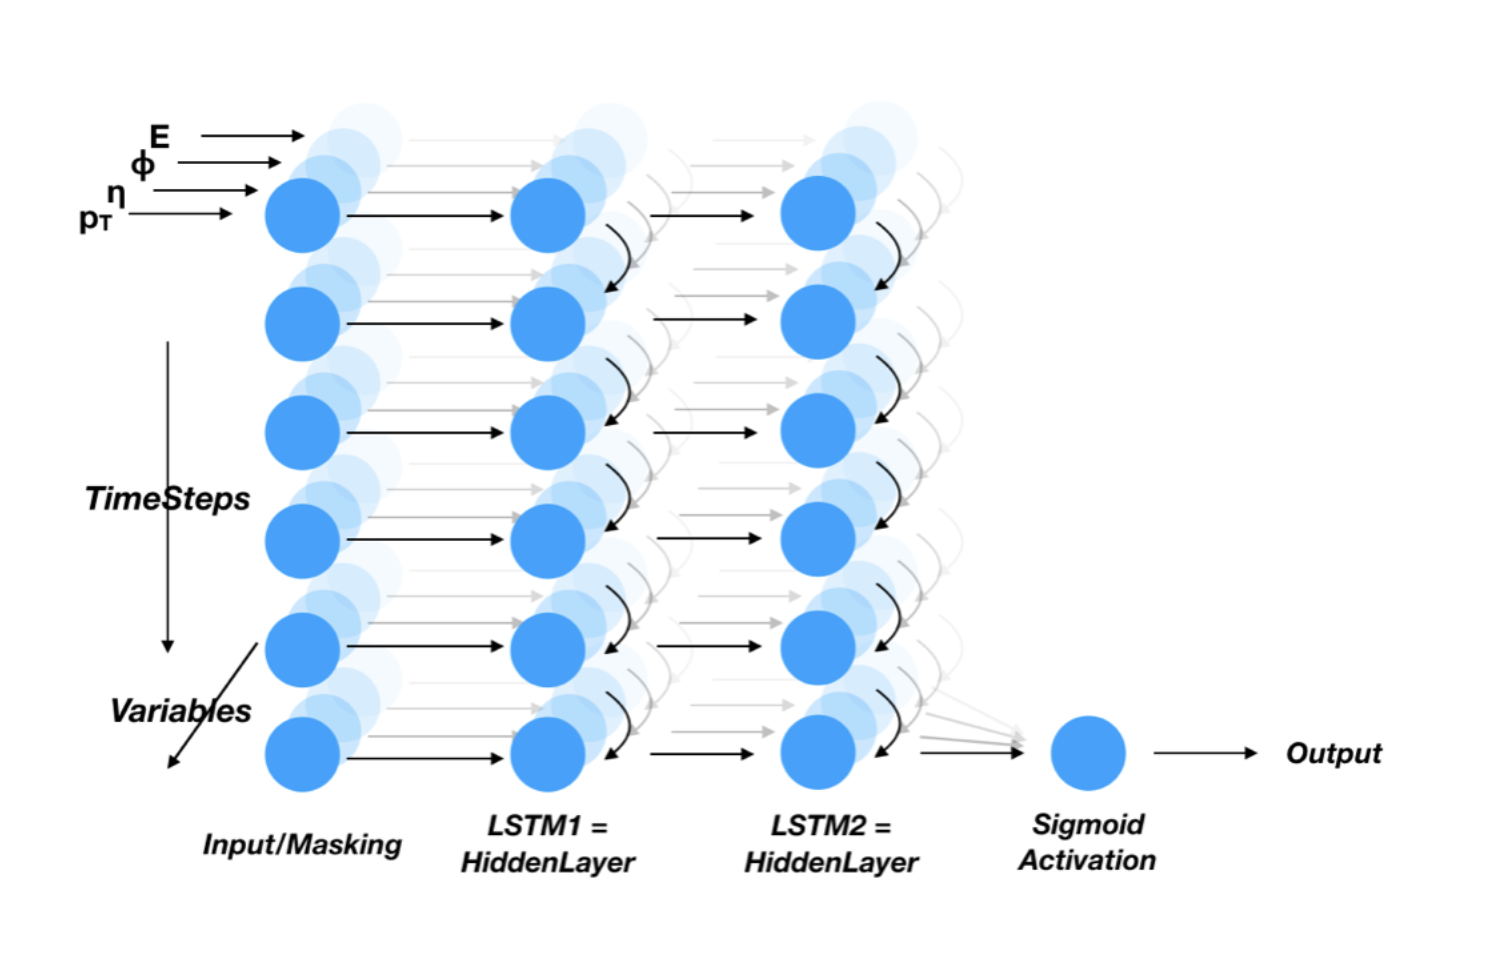
\includegraphics[scale=0.45]{figures/VBFRNN.png}
\caption{Illustration of the VBF-RNN architecture \cite{Antonio_VBFRNN_2023}. The input sequence of jet four-vectors is processed by two stacked LSTM layers, and the final hidden state is passed to a sigmoid output node.}
\label{fig:vbfrnn}
\end{figure}

The network is trained by minimising the binary cross-entropy loss over mini-batches of labelled Monte Carlo events. The available dataset is partitioned into statistically independent training and validation samples; only the training sample contributes to parameter updates, while the validation sample is used to monitor performance and select the final network configuration. The VBF-RNN score is used both as a pre-selection requirement to enrich the sample in VBS-topology events, and as one of the input features to the aQGC discriminant described in Section~\ref{sec:mldiscriminant}.

\section{Machine learning based aQGC discriminant}
\label{sec:mldiscriminant}

While the VBF-RNN identifies the characteristic topology of VBS events, the primary goal of this analysis is to maximise sensitivity to anomalous quartic gauge couplings. The discriminating information between aQGC signal and background is distributed across several event-level observables, motivating the use of an MLP to combine them optimally into a single discriminant.

To define a signal-region-like selection for MLP training, a dedicated boson tagger is applied to the large-$R$ jets. The DisCoJet tagger is an ATLAS machine learning based classifier trained to identify large-$R$ jets consistent with hadronic $W$ or $Z$ boson decays using jet substructure observables. A key property of DisCoJet is that it is explicitly decorrelated from the jet mass, achieved by applying the distance correlation (DisCo) technique during training to minimise the statistical dependence between the tagger score and the jet mass. This decorrelation ensures that the tagger score does not sculpt the jet mass distribution, preserving the latter as a useful observable in the analysis.

A signal-region-like selection, referred to as the BTS65 SR-like selection, is defined by requiring a VBF-RNN v3 score above 0.3 and a DisCoJet score above 0.65 for both large-$R$ jets, as summarised in Table~\ref{tab:mlp_selection}; the MLP-based discriminant is trained and evaluated within this selection.

\begin{table}[h]
\centering
\caption{Signal-region-like selection applied for MLP training and evaluation.}
\label{tab:mlp_selection}
\begin{tabular}{ll}
\toprule
Stage & Requirements \\
\midrule
BTS65 SR-like selection
& VBF-RNN v3 score $> 0.3$ \\
& DisCoJet score $> 0.65$ for both large-$R$ jets \\
\bottomrule
\end{tabular}
\end{table}

\subsection{Input features and training samples}

The MLP takes twelve event-level features as input: the transverse momentum, pseudorapidity, azimuthal angle, and invariant mass of each of the two leading large-$R$ signal jets, the VBF-RNN score from version~3 of the tagger, and three multiplicity variables: the number of tagging jets provided to the RNN, the total number of small-$R$ jets, and the number of large-$R$ jets. All features are standardised to zero mean and unit variance prior to training, as discussed in Chapter~\ref{chap:ml}. Normalised distributions of the input variables for representative S0, M0, and T0 aQGC signal samples and the composite background are shown in Figures~\ref{fig:input_distributions} and~\ref{fig:input_distributions_extra}.

\begin{figure}[h]
\centering
\begin{subfigure}[b]{0.24\textwidth}
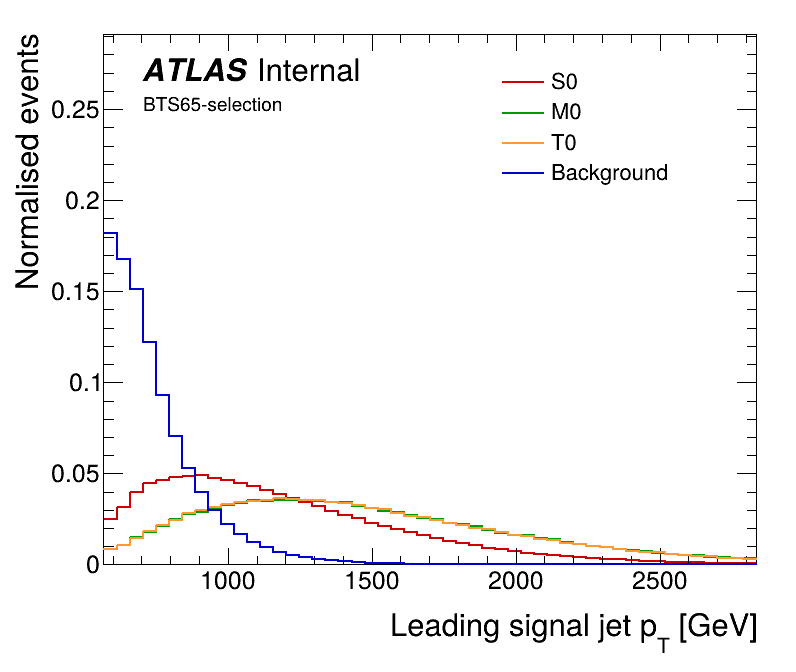
\includegraphics[width=\textwidth]{figures/SigJet1_pT_NOSYS.png}
\end{subfigure}
\begin{subfigure}[b]{0.24\textwidth}
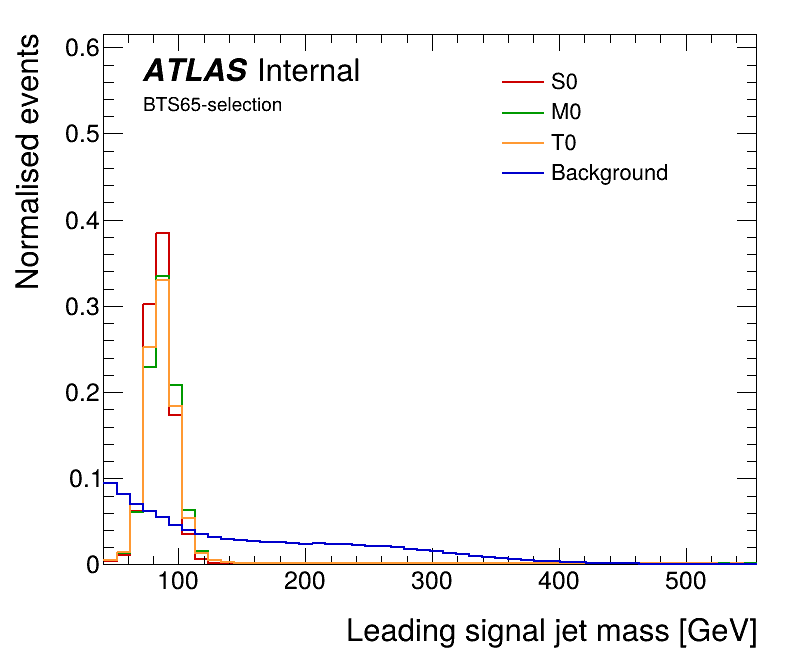
\includegraphics[width=\textwidth]{figures/SigJet1_M_NOSYS.png}
\end{subfigure}
\begin{subfigure}[b]{0.24\textwidth}
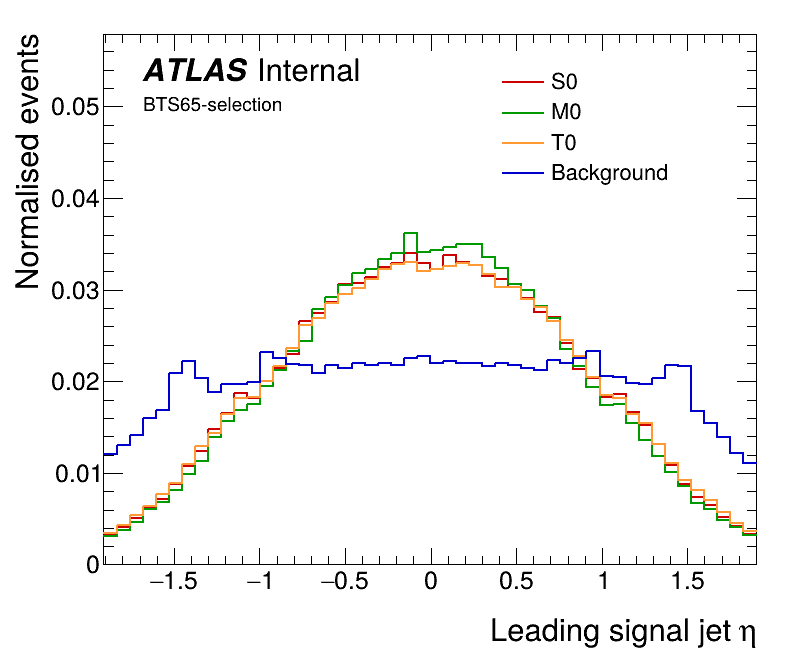
\includegraphics[width=\textwidth]{figures/SigJet1_eta_NOSYS.png}
\end{subfigure}
\begin{subfigure}[b]{0.24\textwidth}
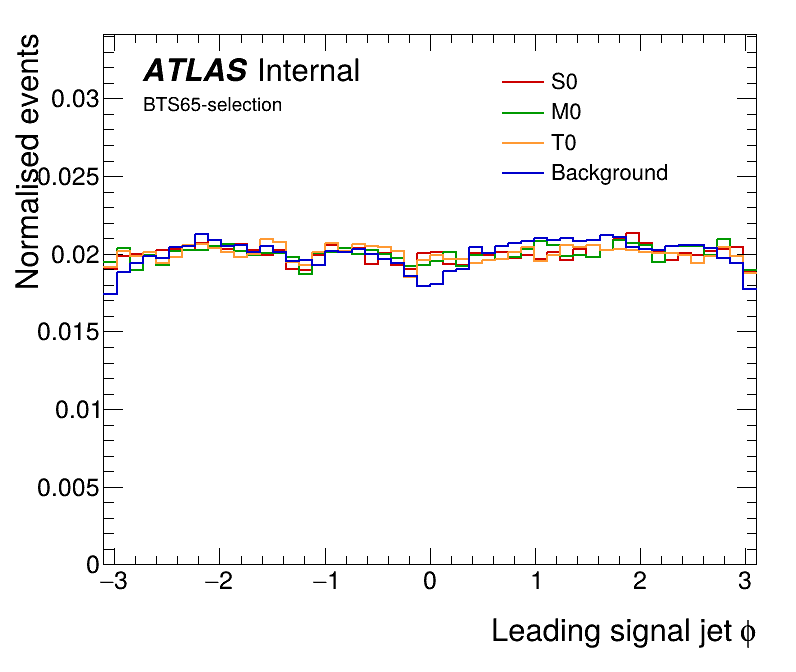
\includegraphics[width=\textwidth]{figures/SigJet1_phi_NOSYS.png}
\end{subfigure}
\begin{subfigure}[b]{0.24\textwidth}
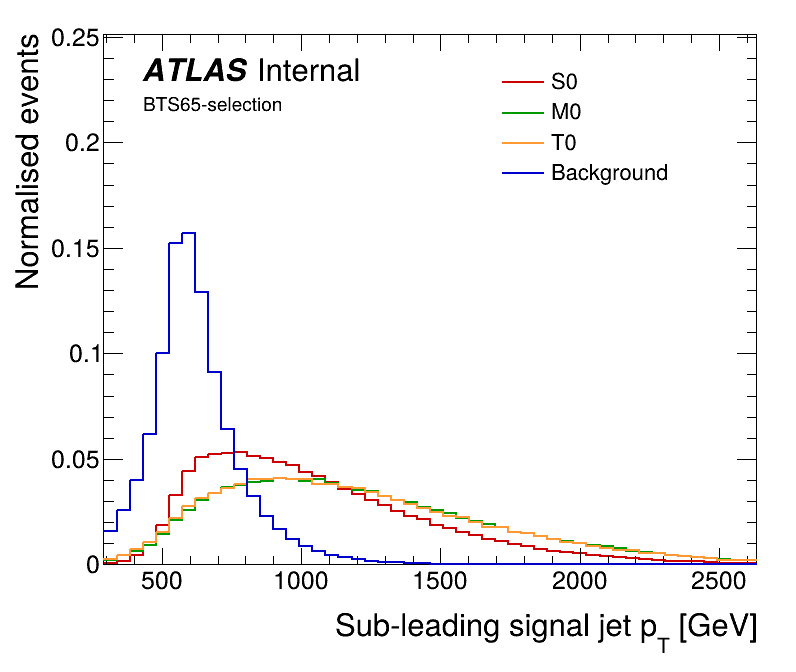
\includegraphics[width=\textwidth]{figures/SigJet2_pT_NOSYS.png}
\end{subfigure}
\begin{subfigure}[b]{0.24\textwidth}
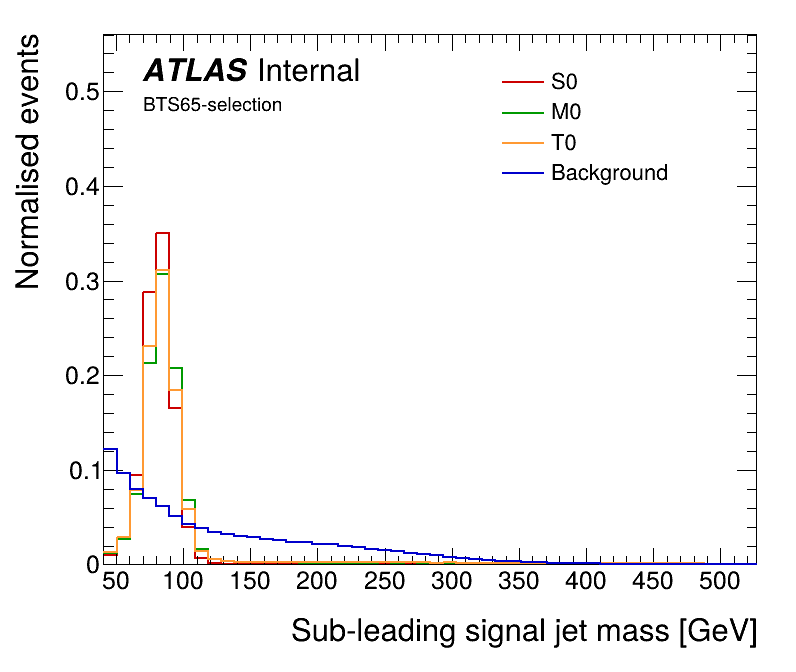
\includegraphics[width=\textwidth]{figures/SigJet2_M_NOSYS.png}
\end{subfigure}
\begin{subfigure}[b]{0.24\textwidth}
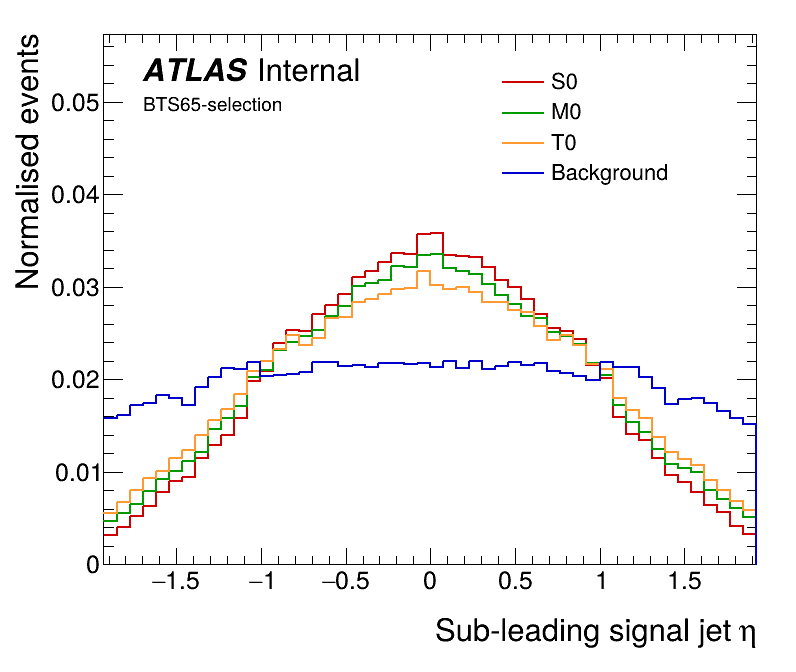
\includegraphics[width=\textwidth]{figures/SigJet2_eta_NOSYS.png}
\end{subfigure}
\begin{subfigure}[b]{0.24\textwidth}
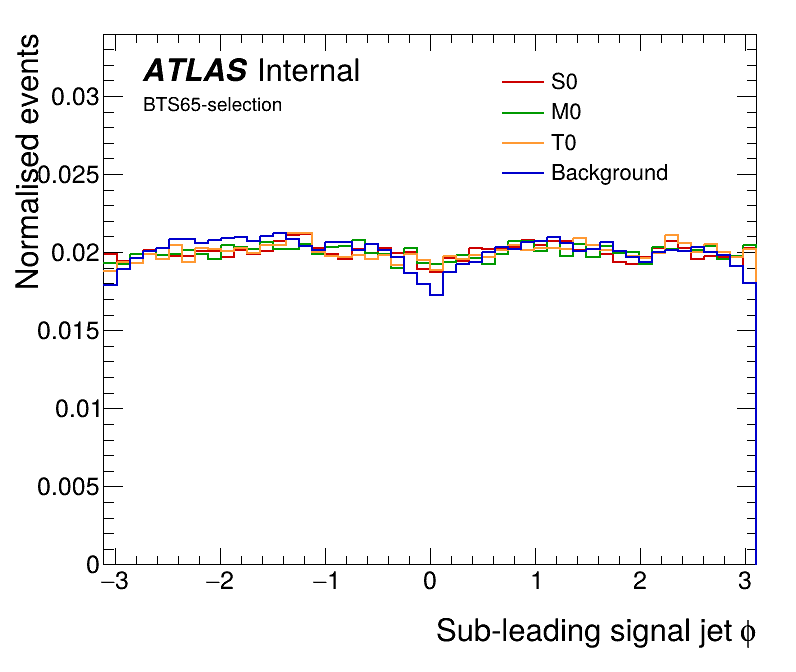
\includegraphics[width=\textwidth]{figures/SigJet2_phi_NOSYS.png}
\end{subfigure}
\caption{Normalised distributions of the eight kinematic MLP input features in the BTS65 SR-like selection. Top row (left to right): leading signal jet $p_T$, mass, $\eta$, and $\phi$. Bottom row: sub-leading signal jet $p_T$, mass, $\eta$, and $\phi$. Distributions are shown for representative S0 (red), M0 (green), and T0 (orange) aQGC signal samples and the composite background (blue). The signal jets are significantly harder and more central than the background, and both jet masses peak near the $W/Z$ boson mass window for signal. The $\phi$ distributions are approximately uniform for all samples, as expected from the azimuthal symmetry of the detector.}
\label{fig:input_distributions}
\end{figure}

\begin{figure}[h]
\centering
\begin{subfigure}[b]{0.24\textwidth}
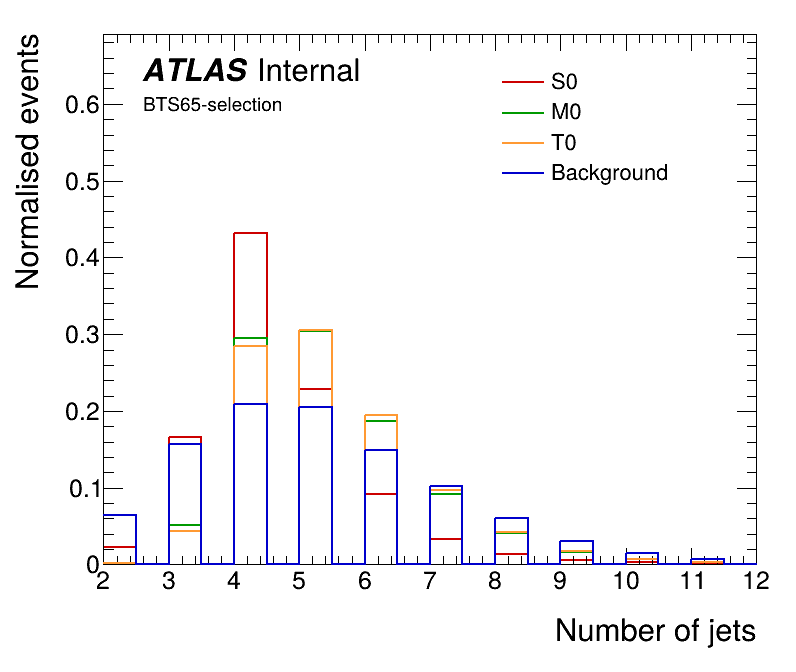
\includegraphics[width=\textwidth]{figures/nJets_NOSYS.png}
\end{subfigure}
\begin{subfigure}[b]{0.24\textwidth}
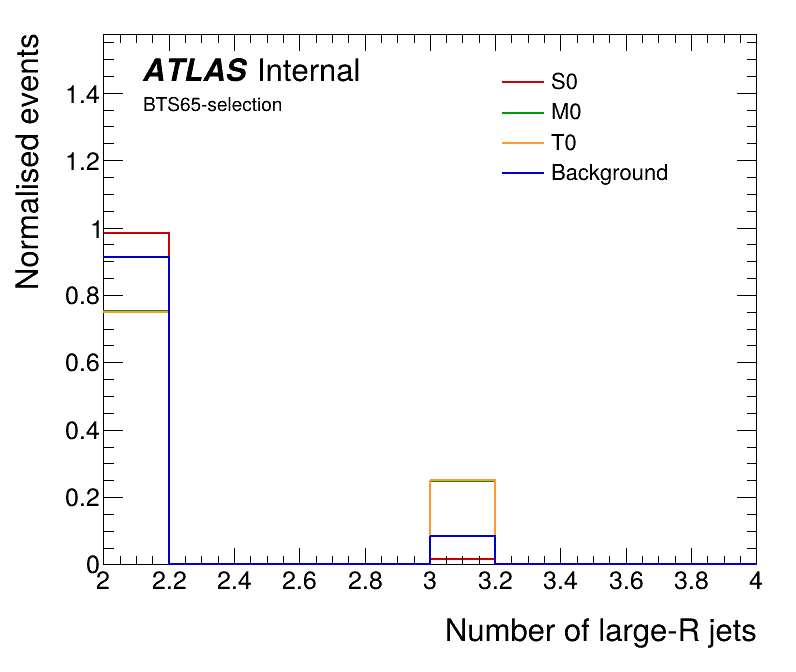
\includegraphics[width=\textwidth]{figures/nLargeRJets_NOSYS.png}
\end{subfigure}
\begin{subfigure}[b]{0.24\textwidth}
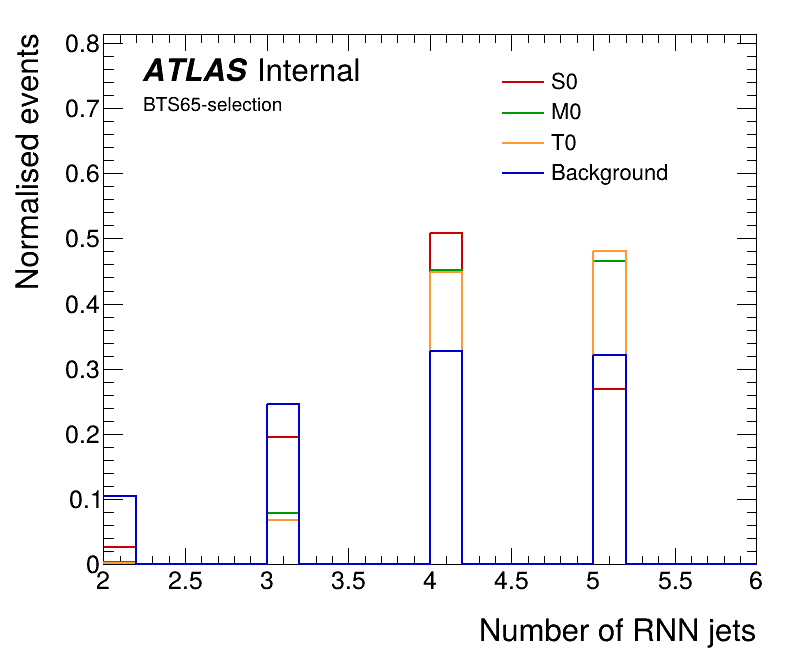
\includegraphics[width=\textwidth]{figures/nRNNJets_NOSYS.png}
\end{subfigure}
\begin{subfigure}[b]{0.24\textwidth}
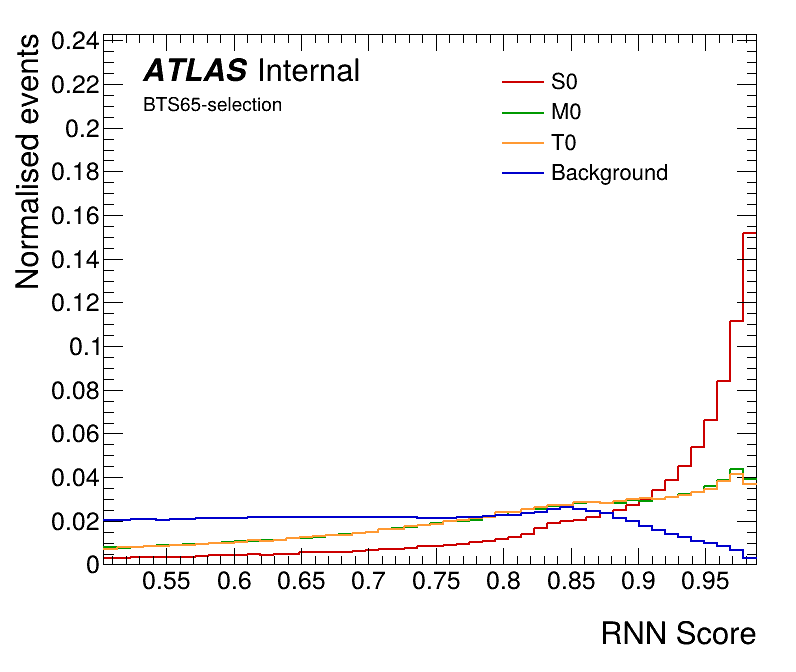
\includegraphics[width=\textwidth]{figures/RNNScore_NOSYS.png}
\end{subfigure}
\caption{Normalised distributions of the jet multiplicity and VBF-RNN input features in the BTS65 SR-like selection. From left to right: total number of small-$R$ jets, number of large-$R$ jets, number of RNN tagging jets, and VBF-RNN score. Distributions are shown for representative S0 (red), M0 (green), and T0 (orange) aQGC signal samples and the composite background (blue). Signal events tend to have higher jet multiplicities and are strongly peaked at high VBF-RNN scores, reflecting their characteristic VBS topology.}
\label{fig:input_distributions_extra}
\end{figure}

The background sample represents the full expected composition in the BTS65 SR-like selection, dominated by QCD dijet production ($\sim\!96\%$), with subdominant contributions from $V$+jets ($\sim\!3\%$), $t\bar{t}$ ($\sim\!1\%$), QCD diboson, and electroweak $VV$+$jj$ production. Only the pure EFT (QUAD) contribution to the signal cross section is used during training, as the interference term between the SM and EFT amplitudes is neglected in this analysis. To avoid the training being dominated by operators with large production cross sections, the aQGC signal samples are reweighted during training so that each operator contributes equally, effectively equalising their cross sections; the correct physical cross sections are restored when evaluating sensitivity. Physical Monte Carlo weights are applied throughout.

\subsection{Binary classifier}

The binary classifier is an MLP with a single sigmoid output node, trained to assign a score $s \in [0,1]$ representing the probability that an event originates from aQGC signal. As discussed in Chapter~\ref{chap:ml}, the sigmoid activation together with the binary cross-entropy loss drives the network output towards the true posterior $P(y=1 \mid \mathbf{x})$.

Two variants of the binary classifier are trained. Specialised models are trained on a single operator family at a time, pairing the two lowest-index operators within each family: $\mathcal{O}_{S,0}+\mathcal{O}_{S,1}$, $\mathcal{O}_{M,0}+\mathcal{O}_{M,1}$, or $\mathcal{O}_{T,0}+\mathcal{O}_{T,1}$. A global model is trained on an ensemble of all available operators spanning the scalar, mixed, and tensor families, $S(0\text{--}1) + M(0\text{--}5,\,7) + T(0\text{--}2,\,5\text{--}9)$, providing broad sensitivity across the full operator space without requiring a separate model for each operator.

\subsection{Multi-class classifier}

The binary approach assigns a single signal probability without distinguishing between operator families. Since the three operator families produce distinct kinematic signatures, as discussed in Chapter~\ref{chap:sm}, a natural extension is to train a single model that simultaneously identifies both the presence of aQGC signal and its operator family.

The multi-class classifier extends the output layer to $K=4$ nodes corresponding to background, scalar, mixed, and tensor classes. A softmax activation is applied to produce a valid probability distribution $(\hat{y}_1,\dots,\hat{y}_K)$ over the four classes, and the network is trained by minimising the categorical cross-entropy loss, following the multi-class formulation described in Chapter~\ref{chap:ml}. The network is trained on all available operators across all three families simultaneously, with class balancing applied to account for the differing numbers of operators per family.

\subsection{Final discriminant and significance estimation}

The final discriminant used for sensitivity estimation is the logarithm of the likelihood ratio derived from the classifier output,
\begin{equation}
D = \log\frac{p_{\mathrm{signal}}}{p_{\mathrm{background}}},
\end{equation}
where $p_{\mathrm{signal}}$ and $p_{\mathrm{background}}$ are the relevant output probabilities from the trained network. For the binary classifier this reduces to the logit transformation of the output score. This transformation is motivated by the Neyman--Pearson lemma, which guarantees that the likelihood ratio is the most powerful test statistic for a simple hypothesis test; by training the classifier to approximate the posterior probabilities, the logit of the output approximates the log-likelihood ratio and therefore approaches the optimal discriminant.

The discriminant is evaluated per individual operator across all model types and binned to form the final template used for sensitivity estimation. The expected sensitivity is quantified using the Asimov binned significance,
\begin{equation}
Z_A = \sqrt{2\sum_i\left[(s_i + b_i)\ln\left(1 + \frac{s_i}{b_i}\right) - s_i\right]},
\end{equation}
where $s_i$ and $b_i$ are the signal and background yields in bin $i$. Results are presented normalised to the significance obtained from the dijet invariant mass $m_{JJ}$ alone, which serves as the baseline discriminant.